\documentclass[11pt,a4paper]{article}

\usepackage[T1]{fontenc}
\usepackage[utf8]{inputenc}
\usepackage{lmodern}
\usepackage{geometry}
\usepackage{microtype}
\usepackage{graphicx}
\usepackage{hyperref}
\usepackage{tikz}
\usetikzlibrary{arrows.meta,positioning,shapes.geometric,fit,backgrounds}

\geometry{margin=0.65in}
\hypersetup{colorlinks=true,linkcolor=blue,urlcolor=blue}

\newcommand{\code}[1]{\texttt{\detokenize{#1}}}

\tikzset{
  block/.style={
    rectangle,
    rounded corners=2pt,
    draw=black!70,
    fill=blue!7,
    align=center,
    minimum height=9mm,
    text width=36mm,
    font=\small
  },
  wideblock/.style={
    block,
    text width=52mm
  },
  smallblock/.style={
    block,
    text width=29mm,
    font=\footnotesize
  },
  decision/.style={
    diamond,
    aspect=2.1,
    draw=black!70,
    fill=orange!12,
    align=center,
    inner sep=1.5pt,
    text width=26mm,
    font=\small
  },
  group/.style={
    rectangle,
    rounded corners=3pt,
    draw=black!40,
    fill=gray!5,
    inner sep=7pt
  },
  arrow/.style={
    -{Latex[length=2.4mm]},
    thick,
    draw=black!75
  },
  dashedarrow/.style={
    arrow,
    dashed,
    draw=black!55
  },
  note/.style={
    rectangle,
    rounded corners=2pt,
    draw=black!45,
    fill=yellow!10,
    align=left,
    text width=130mm,
    font=\small
  }
}

\title{Project Flowcharts for Ship Plate Line Heating}
\author{Ship Plate Bending Line Heating Project}
\date{\today}

\begin{document}
\maketitle

\section*{Purpose}
This document collects the main workflow diagrams for the ship-plate line-heating project: overall software architecture, a single coupled simulation, Li et al. 2023 validation, publication generation, optional research branches, and inverse line-heating planning.

\section{Overall Project Architecture}

\begin{center}
\resizebox{\textwidth}{!}{%
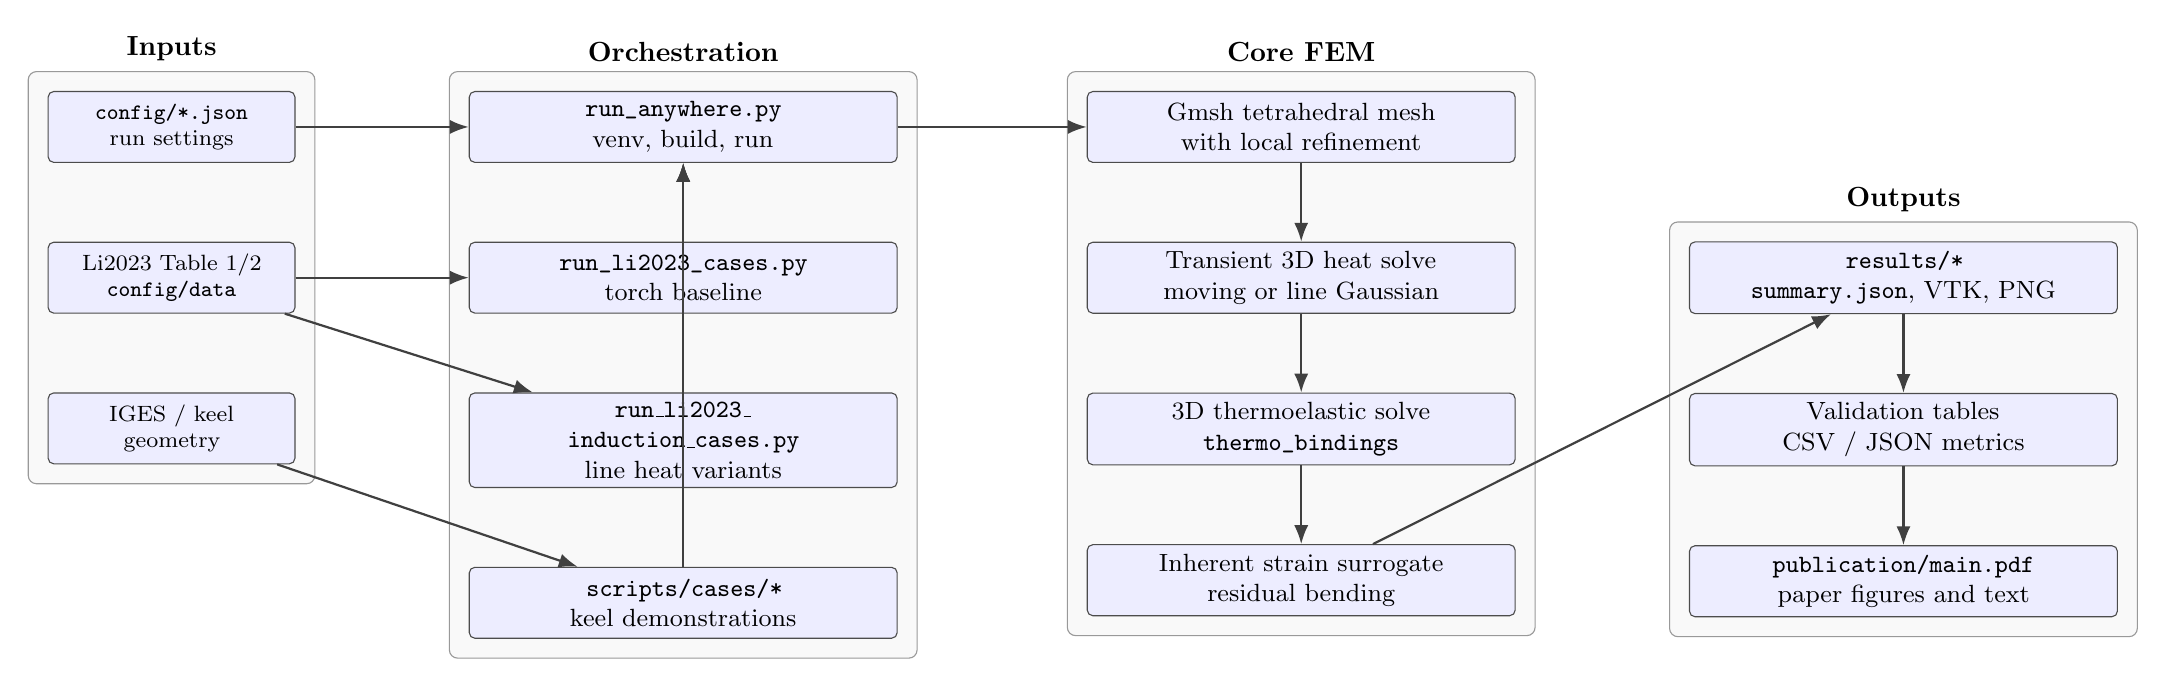
\begin{tikzpicture}[node distance=10mm and 13mm]
  \node[smallblock] (cfg) {\code{config/*.json}\\run settings};
  \node[smallblock, below=of cfg] (li) {Li2023 Table 1/2\\\code{config/data}};
  \node[smallblock, below=of li] (iges) {IGES / keel\\geometry};

  \node[wideblock, right=22mm of cfg] (ra) {\code{run_anywhere.py}\\venv, build, run};
  \node[wideblock, below=of ra] (li23) {\code{run_li2023_cases.py}\\torch baseline};
  \node[wideblock, below=of li23] (ind) {\texttt{run\_li2023\_}\\\texttt{induction\_cases.py}\\line heat variants};
  \node[wideblock, below=of ind] (keel) {\code{scripts/cases/*}\\keel demonstrations};

  \node[wideblock, right=24mm of ra] (mesh) {Gmsh tetrahedral mesh\\with local refinement};
  \node[wideblock, below=of mesh] (heat) {Transient 3D heat solve\\moving or line Gaussian};
  \node[wideblock, below=of heat] (mech) {3D thermoelastic solve\\\code{thermo_bindings}};
  \node[wideblock, below=of mech] (inh) {Inherent strain surrogate\\residual bending};

  \node[wideblock, right=22mm of heat] (res) {\code{results/*}\\\code{summary.json}, VTK, PNG};
  \node[wideblock, below=of res] (val) {Validation tables\\CSV / JSON metrics};
  \node[wideblock, below=of val] (pub) {\code{publication/main.pdf}\\paper figures and text};

  \begin{scope}[on background layer]
    \node[group, fit=(cfg)(li)(iges), label={[font=\bfseries]above:Inputs}] {};
    \node[group, fit=(ra)(li23)(ind)(keel), label={[font=\bfseries]above:Orchestration}] {};
    \node[group, fit=(mesh)(heat)(mech)(inh), label={[font=\bfseries]above:Core FEM}] {};
    \node[group, fit=(res)(val)(pub), label={[font=\bfseries]above:Outputs}] {};
  \end{scope}

  \draw[arrow] (cfg) -- (ra);
  \draw[arrow] (li) -- (li23);
  \draw[arrow] (li) -- (ind);
  \draw[arrow] (iges) -- (keel);
  \draw[arrow] (li23) -- (ra);
  \draw[arrow] (ind) -- (ra);
  \draw[arrow] (keel) -- (ra);
  \draw[arrow] (ra) -- (mesh);
  \draw[arrow] (mesh) -- (heat);
  \draw[arrow] (heat) -- (mech);
  \draw[arrow] (mech) -- (inh);
  \draw[arrow] (inh) -- (res);
  \draw[arrow] (res) -- (val);
  \draw[arrow] (val) -- (pub);
\end{tikzpicture}
}
\end{center}

\section{Single Coupled Simulation Flow}

\begin{center}
\resizebox{\textwidth}{!}{%
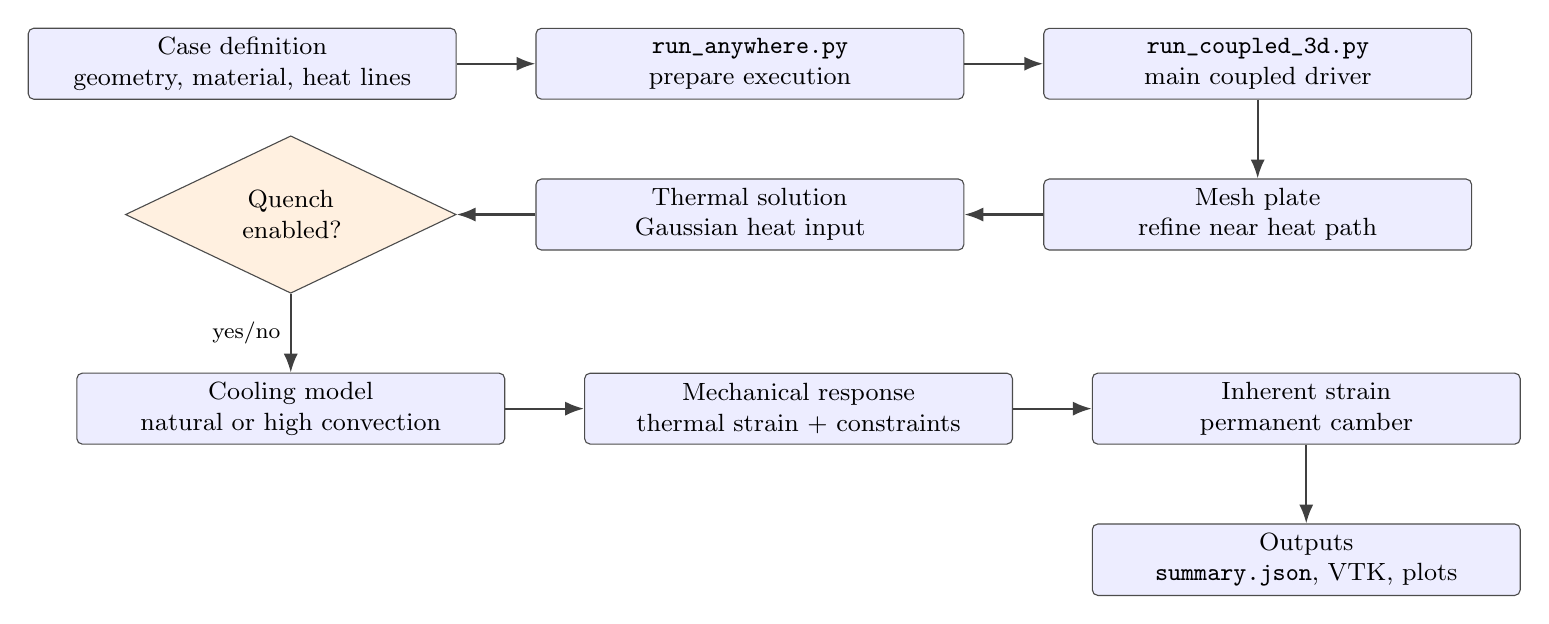
\begin{tikzpicture}[node distance=10mm and 10mm]
  \node[wideblock] (case) {Case definition\\geometry, material, heat lines};
  \node[wideblock, right=of case] (runner) {\code{run_anywhere.py}\\prepare execution};
  \node[wideblock, right=of runner] (solver) {\code{run_coupled_3d.py}\\main coupled driver};

  \node[wideblock, below=of solver] (mesh) {Mesh plate\\refine near heat path};
  \node[wideblock, left=of mesh] (thermal) {Thermal solution\\Gaussian heat input};
  \node[decision, left=of thermal] (quench) {Quench\\enabled?};
  \node[wideblock, below=of quench] (cool) {Cooling model\\natural or high convection};
  \node[wideblock, right=of cool] (mechanics) {Mechanical response\\thermal strain + constraints};
  \node[wideblock, right=of mechanics] (inherent) {Inherent strain\\permanent camber};
  \node[wideblock, below=of inherent] (out) {Outputs\\\code{summary.json}, VTK, plots};

  \draw[arrow] (case) -- (runner);
  \draw[arrow] (runner) -- (solver);
  \draw[arrow] (solver) -- (mesh);
  \draw[arrow] (mesh) -- (thermal);
  \draw[arrow] (thermal) -- (quench);
  \draw[arrow] (quench) -- node[left,font=\footnotesize] {yes/no} (cool);
  \draw[arrow] (cool) -- (mechanics);
  \draw[arrow] (mechanics) -- (inherent);
  \draw[arrow] (inherent) -- (out);
\end{tikzpicture}
}
\end{center}

\section{Li2023 Validation and Process Comparison}

\begin{center}
\resizebox{\textwidth}{!}{%
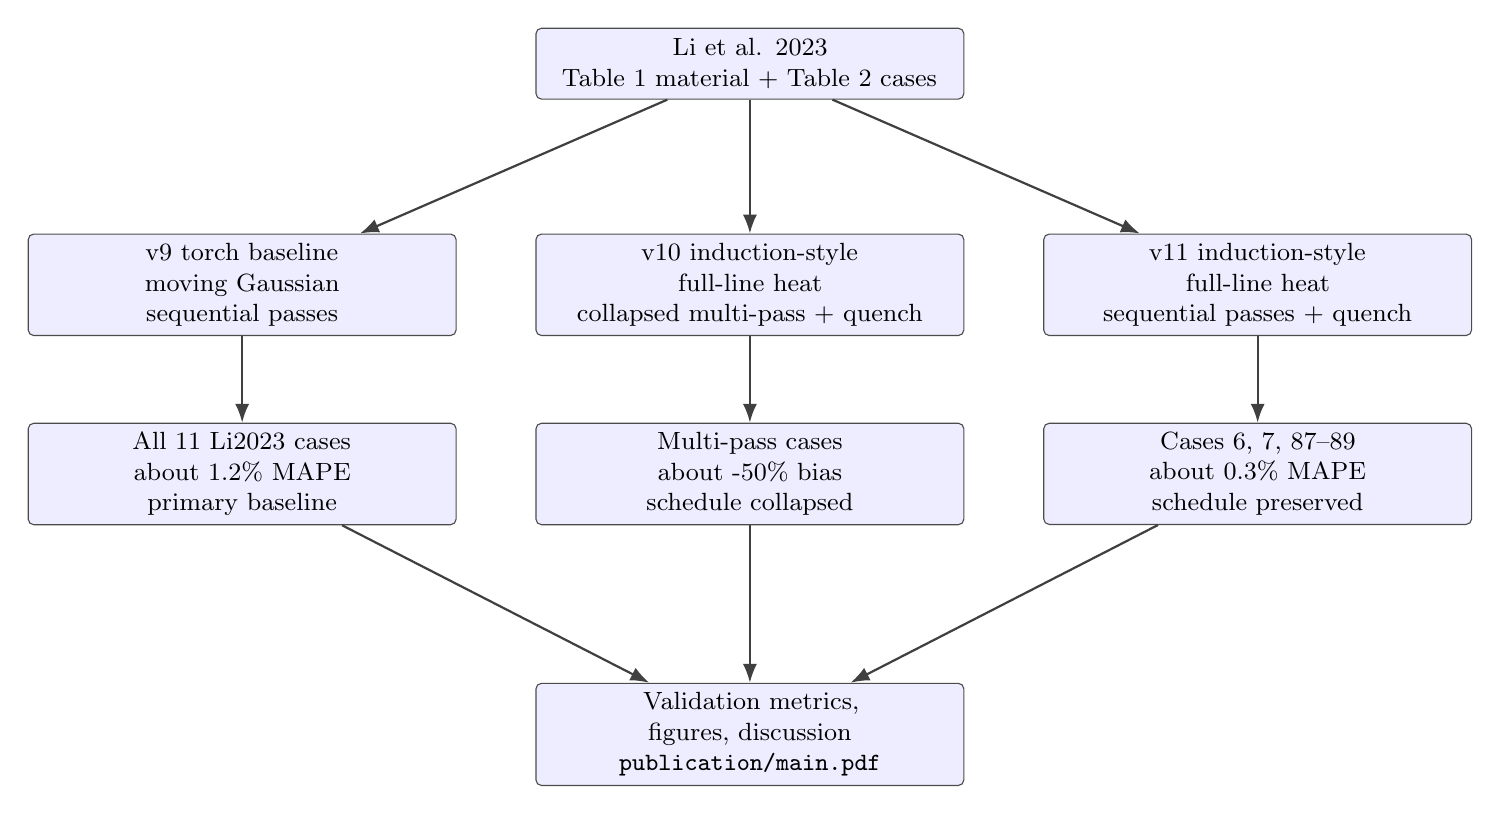
\begin{tikzpicture}[node distance=11mm and 13mm]
  \node[wideblock] (data) {Li et al. 2023\\Table 1 material + Table 2 cases};

  \node[wideblock, below left=17mm and 10mm of data] (v9) {v9 torch baseline\\moving Gaussian\\sequential passes};
  \node[wideblock, below=17mm of data] (v10) {v10 induction-style\\full-line heat\\collapsed multi-pass + quench};
  \node[wideblock, below right=17mm and 10mm of data] (v11) {v11 induction-style\\full-line heat\\sequential passes + quench};

  \node[wideblock, below=of v9] (r9) {All 11 Li2023 cases\\about 1.2\% MAPE\\primary baseline};
  \node[wideblock, below=of v10] (r10) {Multi-pass cases\\about -50\% bias\\schedule collapsed};
  \node[wideblock, below=of v11] (r11) {Cases 6, 7, 87--89\\about 0.3\% MAPE\\schedule preserved};

  \node[wideblock, below=20mm of r10] (paper) {Validation metrics, figures, discussion\\\code{publication/main.pdf}};

  \draw[arrow] (data) -- (v9);
  \draw[arrow] (data) -- (v10);
  \draw[arrow] (data) -- (v11);
  \draw[arrow] (v9) -- (r9);
  \draw[arrow] (v10) -- (r10);
  \draw[arrow] (v11) -- (r11);
  \draw[arrow] (r9) -- (paper);
  \draw[arrow] (r10) -- (paper);
  \draw[arrow] (r11) -- (paper);
\end{tikzpicture}
}
\end{center}

\begin{center}
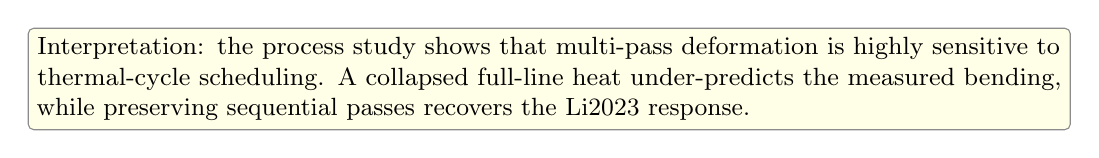
\begin{tikzpicture}
  \node[note] {
    Interpretation: the process study shows that multi-pass deformation is highly sensitive to thermal-cycle scheduling. A collapsed full-line heat under-predicts the measured bending, while preserving sequential passes recovers the Li2023 response.
  };
\end{tikzpicture}
\end{center}

\section{Publication Generation Pipeline}

\begin{center}
\resizebox{\textwidth}{!}{%
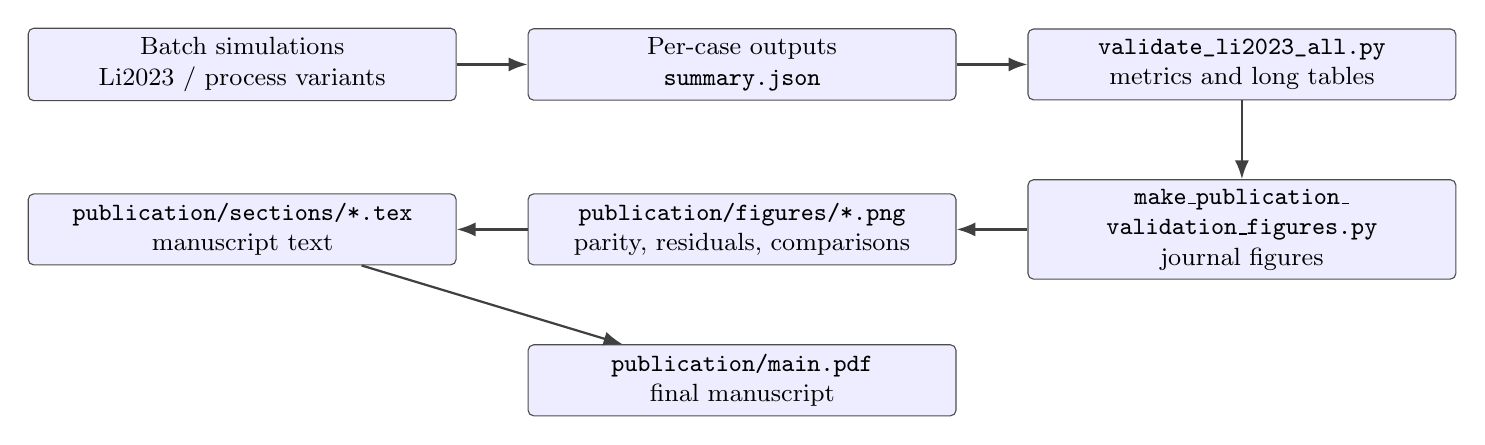
\begin{tikzpicture}[node distance=10mm and 9mm]
  \node[wideblock] (batch) {Batch simulations\\Li2023 / process variants};
  \node[wideblock, right=of batch] (summary) {Per-case outputs\\\code{summary.json}};
  \node[wideblock, right=of summary] (validate) {\code{validate_li2023_all.py}\\metrics and long tables};
  \node[wideblock, below=of validate] (figscript) {\texttt{make\_publication\_}\\\texttt{validation\_figures.py}\\journal figures};
  \node[wideblock, left=of figscript] (png) {\code{publication/figures/*.png}\\parity, residuals, comparisons};
  \node[wideblock, left=of png] (tex) {\code{publication/sections/*.tex}\\manuscript text};
  \node[wideblock, below=of png] (pdf) {\code{publication/main.pdf}\\final manuscript};

  \draw[arrow] (batch) -- (summary);
  \draw[arrow] (summary) -- (validate);
  \draw[arrow] (validate) -- (figscript);
  \draw[arrow] (figscript) -- (png);
  \draw[arrow] (png) -- (tex);
  \draw[arrow] (tex) -- (pdf);
\end{tikzpicture}
}
\end{center}

\section{Inverse Line-Heating Planning Procedure}

\begin{center}
\resizebox{\textwidth}{!}{%
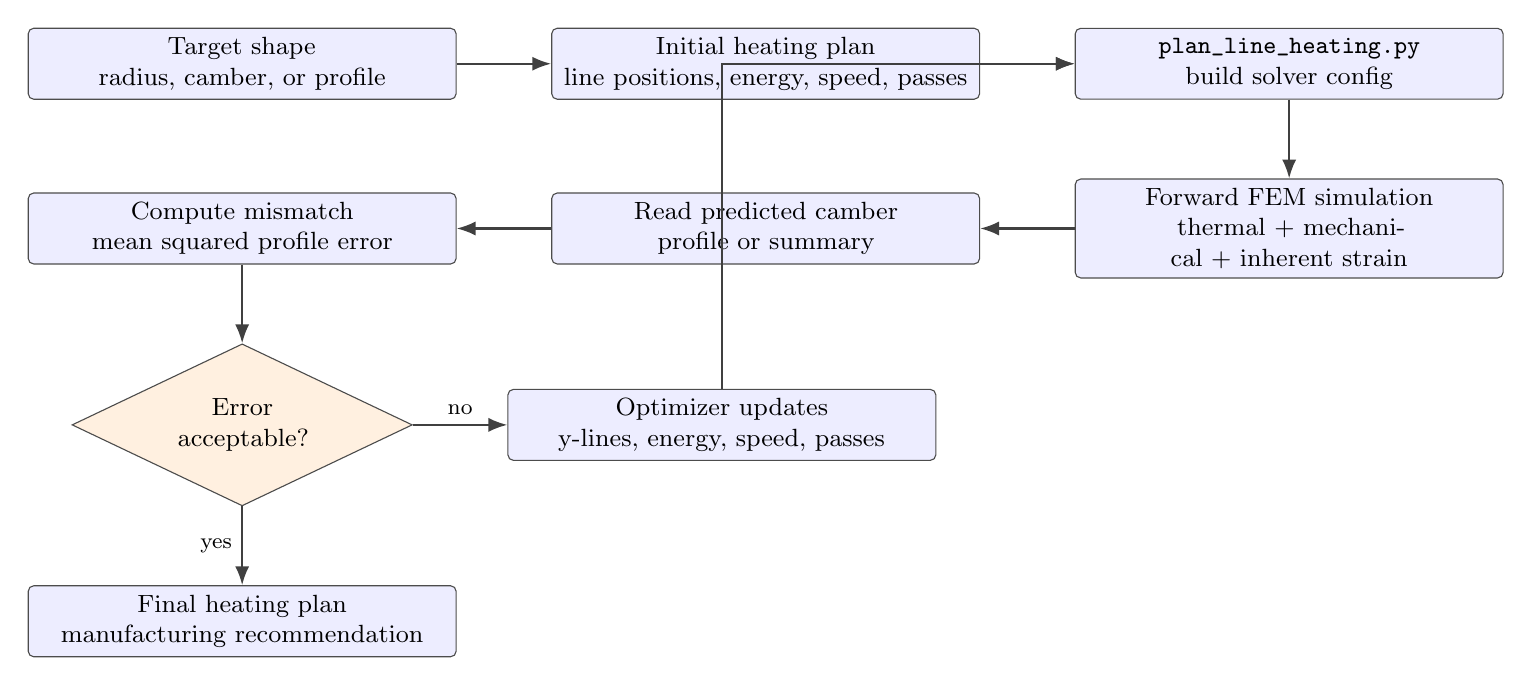
\begin{tikzpicture}[node distance=10mm and 12mm]
  \node[wideblock] (target) {Target shape\\radius, camber, or profile};
  \node[wideblock, right=of target] (guess) {Initial heating plan\\line positions, energy, speed, passes};
  \node[wideblock, right=of guess] (build) {\code{plan_line_heating.py}\\build solver config};
  \node[wideblock, below=of build] (forward) {Forward FEM simulation\\thermal + mechanical + inherent strain};
  \node[wideblock, left=of forward] (read) {Read predicted camber\\profile or summary};
  \node[wideblock, left=of read] (misfit) {Compute mismatch\\mean squared profile error};
  \node[decision, below=of misfit] (ok) {Error\\acceptable?};
  \node[wideblock, right=of ok] (update) {Optimizer updates\\y-lines, energy, speed, passes};
  \node[wideblock, below=of ok] (final) {Final heating plan\\manufacturing recommendation};

  \draw[arrow] (target) -- (guess);
  \draw[arrow] (guess) -- (build);
  \draw[arrow] (build) -- (forward);
  \draw[arrow] (forward) -- (read);
  \draw[arrow] (read) -- (misfit);
  \draw[arrow] (misfit) -- (ok);
  \draw[arrow] (ok) -- node[above,font=\footnotesize] {no} (update);
  \draw[arrow] (update) |- (build);
  \draw[arrow] (ok) -- node[left,font=\footnotesize] {yes} (final);
\end{tikzpicture}
}
\end{center}

\begin{center}
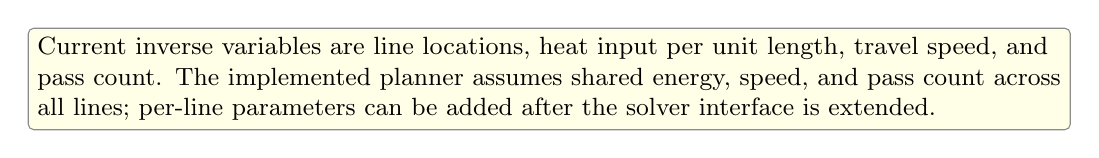
\begin{tikzpicture}
  \node[note] {
    Current inverse variables are line locations, heat input per unit length, travel speed, and pass count. The implemented planner assumes shared energy, speed, and pass count across all lines; per-line parameters can be added after the solver interface is extended.
  };
\end{tikzpicture}
\end{center}

\section{Optional Research and Application Branches}

\begin{center}
\resizebox{\textwidth}{!}{%
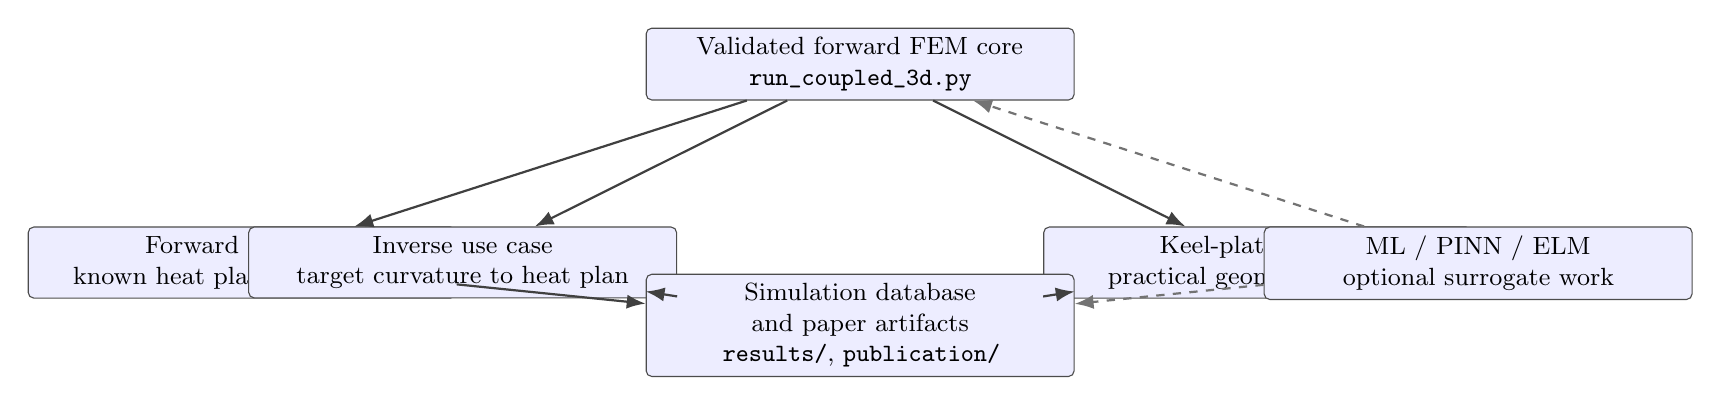
\begin{tikzpicture}[node distance=10mm and 12mm]
  \node[wideblock] (core) {Validated forward FEM core\\\code{run_coupled_3d.py}};

  \node[wideblock, below left=16mm and 24mm of core] (forward) {Forward use case\\known heat plan to curvature};
  \node[wideblock, below left=16mm and -4mm of core] (inverse) {Inverse use case\\target curvature to heat plan};
  \node[wideblock, below right=16mm and -4mm of core] (keel) {Keel-plate demos\\practical geometry studies};
  \node[wideblock, below right=16mm and 24mm of core] (ml) {ML / PINN / ELM\\optional surrogate work};

  \node[wideblock, below=22mm of core] (results) {Simulation database and paper artifacts\\\code{results/}, \code{publication/}};

  \draw[arrow] (core) -- (forward);
  \draw[arrow] (core) -- (inverse);
  \draw[arrow] (core) -- (keel);
  \draw[dashedarrow] (ml) -- (core);
  \draw[arrow] (forward) -- (results);
  \draw[arrow] (inverse) -- (results);
  \draw[arrow] (keel) -- (results);
  \draw[dashedarrow] (ml) -- (results);
\end{tikzpicture}
}
\end{center}

\section{File-Level Map}

\begin{center}
\resizebox{\textwidth}{!}{%
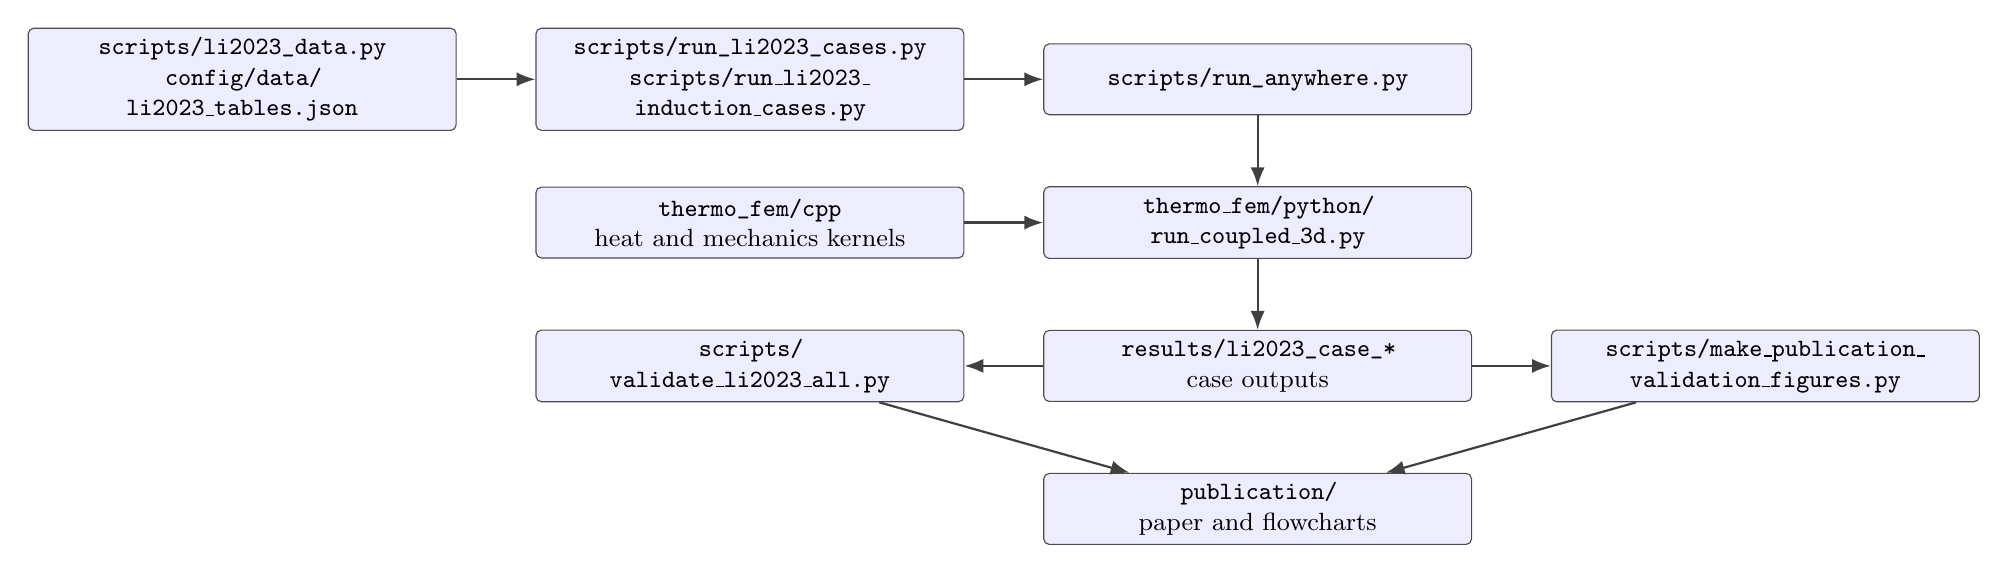
\begin{tikzpicture}[node distance=9mm and 10mm]
  \node[wideblock] (data) {\code{scripts/li2023_data.py}\\\texttt{config/data/}\\\texttt{li2023\_tables.json}};
  \node[wideblock, right=of data] (drivers) {\code{scripts/run_li2023_cases.py}\\\texttt{scripts/run\_li2023\_}\\\texttt{induction\_cases.py}};
  \node[wideblock, right=of drivers] (runner) {\code{scripts/run_anywhere.py}};
  \node[wideblock, below=of runner] (solver) {\texttt{thermo\_fem/python/}\\\texttt{run\_coupled\_3d.py}};
  \node[wideblock, left=of solver] (cpp) {\code{thermo_fem/cpp}\\heat and mechanics kernels};
  \node[wideblock, below=of solver] (results) {\code{results/li2023_case_*}\\case outputs};
  \node[wideblock, left=of results] (validate) {\texttt{scripts/}\\\texttt{validate\_li2023\_all.py}};
  \node[wideblock, right=of results] (figures) {\texttt{scripts/make\_publication\_}\\\texttt{validation\_figures.py}};
  \node[wideblock, below=of results] (publication) {\code{publication/}\\paper and flowcharts};

  \draw[arrow] (data) -- (drivers);
  \draw[arrow] (drivers) -- (runner);
  \draw[arrow] (runner) -- (solver);
  \draw[arrow] (cpp) -- (solver);
  \draw[arrow] (solver) -- (results);
  \draw[arrow] (results) -- (validate);
  \draw[arrow] (results) -- (figures);
  \draw[arrow] (validate) -- (publication);
  \draw[arrow] (figures) -- (publication);
\end{tikzpicture}
}
\end{center}

\end{document}
